% !TEX encoding = UTF-8 Unicode
%!TEX root = thesis.tex
% !TEX spellcheck = en-US
%%=========================================
\chapter{Introduction}

%%=========================================
\section{Background}

%%=========================================
\subsection*{Problem Formulation / Motivation / Purpose?}


%%=========================================
\subsection*{Related work}

{
    \color{BrickRed}
    \begin{itemize}
        \item SphenoBlock

    \end{itemize}
}

%%=========================================
\subsection*{What Remains to be Done?}

%%=========================================
\section{Objectives / Research Questions}
What follow are the research questions which motivates this project: 
\noindent
\textbf{Main RQ:} How can AR support teaching of rat brain anatomy and dissection for medical students?
\begin{itemize}
    \item {
        \textbf{RQ1:} How should interaction in be implemented in AR to accommodate medical professionals?
    }
    \item {
        \textbf{RQ2:} How will a collaborative experience shared between an HMD and a smartphone compare to accommodate medical professionals?
    }
    \item {
        \color{BrickRed}
        \textbf{RQ3: }
        Something about macro + microscopic visualization:
        How should microscopical data be visualized in a macroscopical model to best effect? (WIP)
    }
\end{itemize}


%%=========================================
\section{Approach}


\subsection*{Research method}

\begin{wrapfigure}{R}{0.50\textwidth}
    \begin{center}
        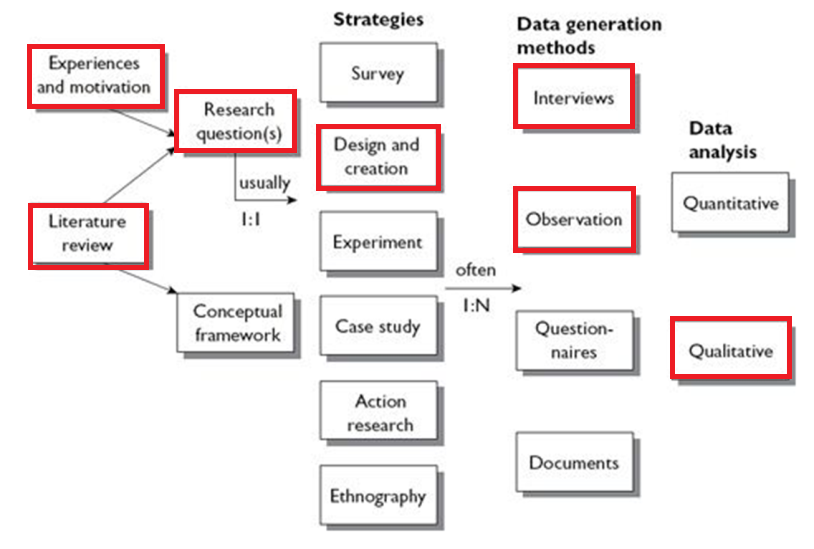
\includegraphics[width=0.45\textwidth]{fig/researchplan_image}
    \end{center}
    \caption{Model of the research process as illustrated in \citep{oates2006} }
    \label{researchplan_img}
\end{wrapfigure}

The research questions were derived through discussing the needs of the intended users with neuroscientists at the Kavli Institute. It was then narrowed down by a literature review, finding a lack of satisfactory substitutions for real brain dissections and especially finding no attempt at a practical multiplatform application for a more scalable use for students. The projects research question falls under the strategy of Design and Creation as the main goal is to develop a useful application for medical education. The focus on a smartphone solution was further motivated by the COVID-pandemic making from-home learning quite essential and making the passing around of HMD devices an unwanted scenario. As part of an agile software development model the gathering of qualitative data from observations and interviews within the scope of user testing will be essential. 

\subsection*{Development method}

\section{Contributions}
%% write about macro vs micro stuff

The research product resulting from this project will be a new computer-based software application using augmented reality and running on multiple platforms like HoloLens 1 and 2, Android and more. The aim will be to develop an application that can bridge the gap between expensive head mounted displays and everyday smartphones which you will find in the pocket of any student, and to use this as a collaborative tool for learning neuroanatomy. Throughout the development period we will consult with medical professionals and gather feedback from students on the usability of the application.

{
    \color{BrickRed}
    \noindent
    \newline
    Something about macro + micro
}

%%=========================================
\section{Limitations}

%%=========================================
\section{Outline}

